
%%%%%%%%%%%%%%%%%%%%%%%%%%%%%%%%%%%%%%%%%%%% Articolo - A4 - Landscape


%%%%%%%%%%%%%%%%%%%%%%%%%%%%%%%%%%%%%%%%%%%% preambolo

\documentclass[11pt, landscape]{article}
\usepackage[utf8]{inputenc}
\usepackage[italian]{babel}
\usepackage{multicol}
\usepackage{caption}
\captionsetup{justification   = raggedright,
              singlelinecheck = false}
\setlength{\columnsep}{1cm}
\usepackage[margin=1in]{geometry}
\usepackage{amsfonts, amsmath, amssymb}
\usepackage[none]{hyphenat}
\usepackage{fancyhdr}
\usepackage{graphics}
\usepackage{graphicx}
\usepackage[export]{adjustbox}
\usepackage{float}
\usepackage[nottoc, notlot, notlof]{tocbibind}
\usepackage{pgf,tikz,pgfplots} 
\pgfplotsset{compat=1.15}
\usepackage{mathrsfs}
\usetikzlibrary{arrows}

\pagestyle{fancy}
\fancyhead{}
\fancyfoot{}
\fancyhead[L]{\small \MakeUppercase{Spunti di matematica}}
\fancyhead[C]{\small \emph{classe 5QA}}
\fancyhead[R]{\small \emph{prof. Diego Fantinelli}}

\fancyfoot[C]{\thepage}
\renewcommand{\headrulewidth}{0.5pt}
\renewcommand{\footrulewidth}{0.1pt}

\parindent 0ex
\setlength{\parindent}{4em}
\setlength{\parskip}{1em}
\renewcommand{\baselinestretch}{1.5}

%%%%%%%%%%%%%%%%%%%%%%%%%%%%%%%%%%%%%%%%%%%% title page

\begin{document}

\begin{titlepage}
\begin{center}
\vspace*{1cm}
\Large{\textbf{IIS "GA REMONDINI" - Bassano del Grappa}}\\
\Large{\textbf{Anno Scolastico 2020/'21}}\\
\vfill
\line(1,0){400}\\[.5mm]
\huge{\textbf{SPUNTI DI MATEMATICA}}\\[3mm]
\Large{\textbf{per il colloquio finale dell'Esame di Stato}}\\
\line(1,0){400}\\
\vfill
{\em prof. Diego Fantinelli}\\
{Classe 5QA } \\
%{\scriptsize \today} \\

\end{center}
\end{titlepage}

%%%%%%%%%%%%%%%%%%%%%%%%%%%%%%%%%%%%%%%%%%%% introduzione

%\tableofcontents
%\thispagestyle{empty}
%\clearpage

\setcounter{page}{1}

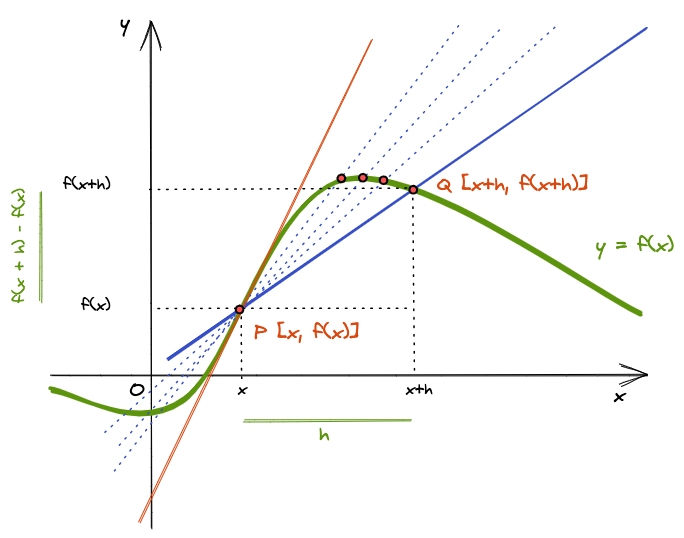
\includegraphics[width=0.9\textwidth]{derivata_01.png}

\begin{figure}
\setlength{\fboxrule}{0.7pt}
\fbox{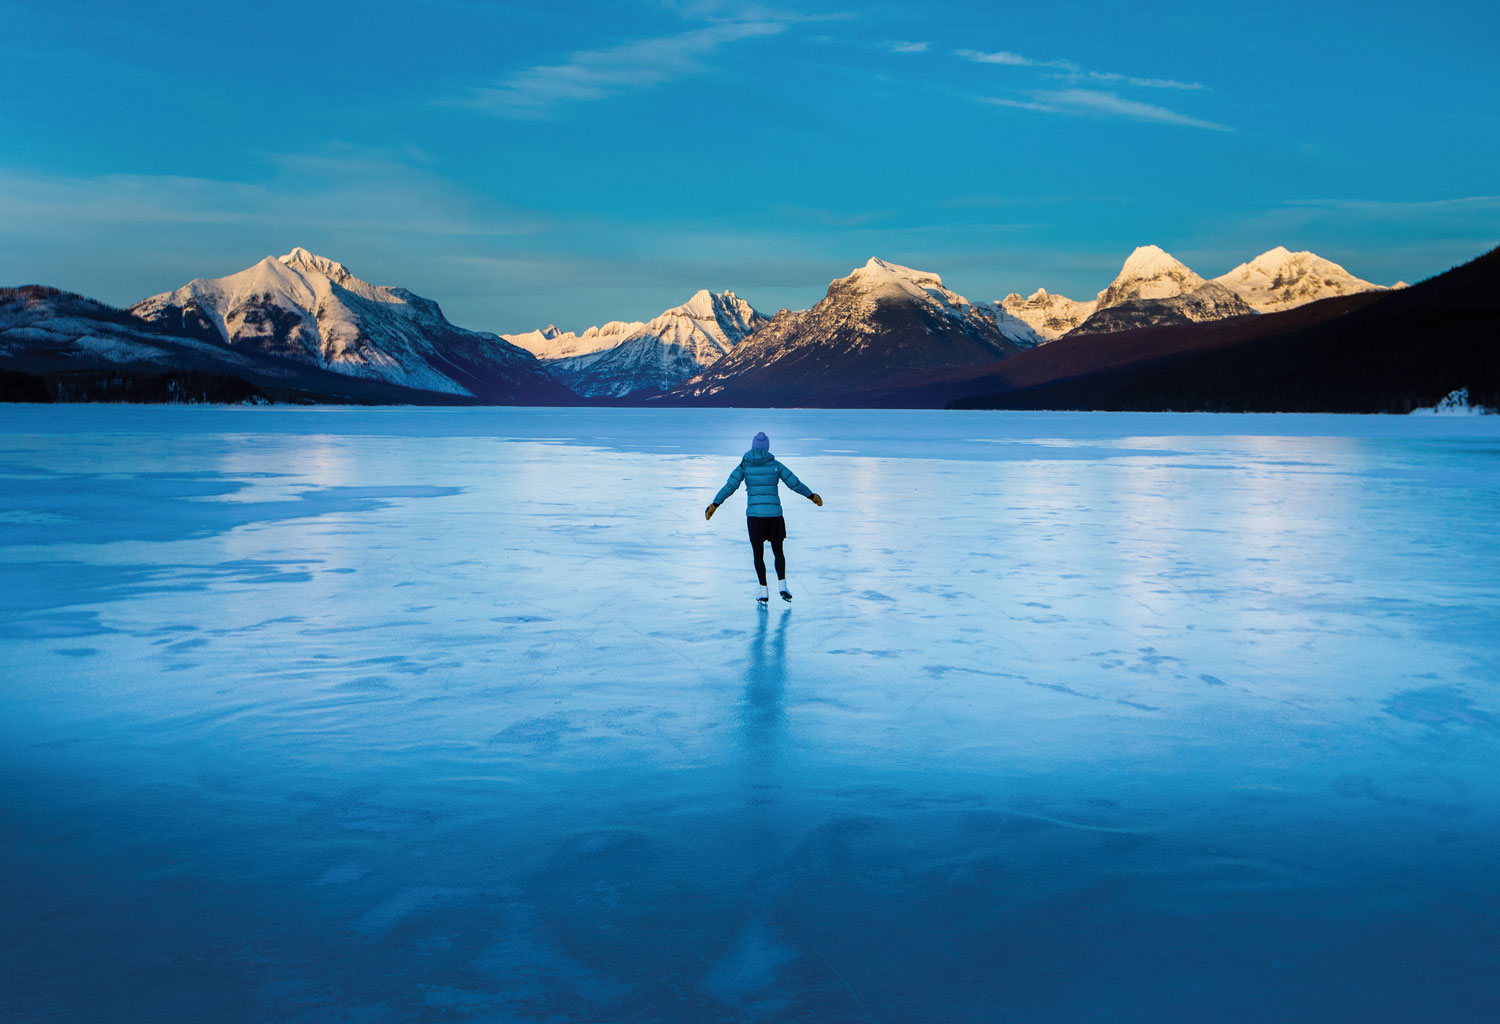
\includegraphics[width=\textwidth]{ice.png}}
\end{figure}

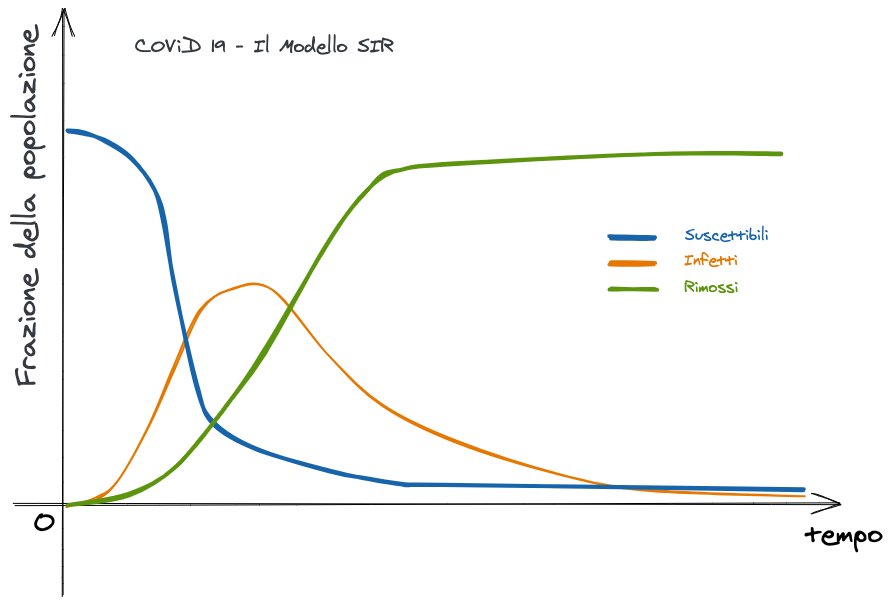
\includegraphics[width=\textwidth]{covid.png}

\end{document}
